\section{Introduction}

%{\bf Previous content:}
%
%This report describes a new model for optimised traffic signal
%planning using a MILP formulation. Previously,
%\trbcite{lin2004enhanced} describe a MILP formulation for optimised
%traffic signal planning based on the Cell Transmission Model of
%\trbcite{daganzo1995cell}. However a CTM based model is limited in
%scalability by the requirement that each road way in the network must
%be partitioned up into segments that take exactly $\DT[]=1$ to
%traverse at the free flow speed. We get around this limitation by
%using a queue based model that supports non-homogeneous time steps,
%and we will show how we can exploit this property to scale a network
%without significant increase in the number of variables or loss of
%quality.
%
%{\bf Scott's suggested argument structure:}
%
%\remark{I say we drop the issue of many segments and simply criticize
%  the CTM by saying that it is not easy to make non-homogeneous and
%  that is what we need?  In general, the Intro probably has to push on
%  the non-homogeneous motivation a little earlier and forcefully since
%  we're claiming *this* is the reason for the paper, the QTM and
%  ultimately our evaluation comparing homogeneous vs. non-homogeneous.
%  We may have broader (not fully validated) motivations but we need a
%  watertight argument and paper.}

As urban traffic congestion is on the increase worldwide with
estimated productivity losses in the hundreds of billions of dollars
in the U.S. alone and immeasurable environmental
impact~\cite{bazzan2013intro}, it is critical to maximize capacity and
throughput of existing road infrastructure through optimized traffic
signal control.  Unfortunately, many large cities still use some
degree of \emph{fixed-time} control~\trbcitenum{el2013multiagent} even
if they also use \emph{actuated} or \emph{adaptive} control methods
such as SCATS~\trbcitenum{scats80} or SCOOT~\trbcitenum{scoot81}.
However, there is further opportunity to improve traffic signal
control even beyond adaptive methods through the use of
\emph{optimized} controllers as evidenced in a variety of approaches
ranging from mixed integer (linear)
programming~\trbcitenum{gartner1974optimization,gartner2002arterial,lo1998novel,he2011pamscod,lin2004enhanced,han2012link}
to heuristic search~\trbcitenum{lo1999dynamic,he2010heuristic} to
scheduling~\trbcitenum{smith2013surtrac} to reinforcement
learning~\trbcitenum{el2013multiagent}.  Such optimized
controllers hold the promise of maximizing existing infrastructure
capacity by finding more complex (and potentially closer to optimal)
jointly coordinated intersection policies in comparison to
heuristically-adaptive policies such as SCATS and SCOOT. 
%master-slave approaches such as SCATS and SCOOT, such optimized methods
However, optimized methods are computationally demanding 
%compared to adpative control methods such as SCOOT and SCATS
%(which can run on 1970's error hardware)
and often do not guarantee \emph{jointly} optimal solutions over a
large intersection network either because (a) they only consider
coordination of neighboring intersections or arterial routes or (b)
they fail to scale to large intersection networks simply for
computational reasons.  We remark that the latter scalability issue is endemic
to many mixed integer programming approaches to optimized signal control.

In this work, we build on the body of work in mixed integer linear
programming (MILP) approaches that attempt to jointly optimize traffic
signal control over an \emph{entire traffic network}~(rather than
focus on arterial routes) and specifically on improving the
scalability of these methods for large urban traffic networks.  In our
investigation of existing approaches in this vein, namely exemplar
methods in the spirit of~\trbcitenum{lo1998novel,lin2004enhanced,han2012link} that
use a (modified) cell transmission model
(CTM)~\trbcitenum{daganzo1994cell,daganzo1995cell} for their underlying
prediction of traffic flows, we remark that a major drawback is the
CTM-imposed requirement to choose a predetermined \emph{homogeneous} (and
often necessarily small) time step for reasonable modeling fidelity.
This need to model a large number of CTM cells with a small time step
leads to MILPs that are exceedingly large and often intractable to
solve. %% FWT: seems redundant "for large traffic networks."

Our primary insight in this work stems from the fact that MILP-based
approaches to traffic control used in a receding horizon control
manner (that replan at fixed time intervals) need to compute high
fidelity control policies only for the early stages of the signal
plan; therefore, coarser time steps can be employed to ``see'' over a
long horizon to preemptively adapt to distant platoons and other
predicted long-term changes in traffic flows.
This need for non-homogeneous control in
turn spawns the need for an additional innovation: we require a
traffic flow
%% FWT: "simulation" here is confusing in my opinion.
model that permits non-homogeneous time steps and properly models the
travel time delay between lights.  To this end, we might consider CTM
extensions such as the variable cell length
CTM~\trbcitenum{xiaojian2010urban}, stochastic CTM
~\trbcitenum{sumalee2011stochastic,jabari2012stochastic},
CTM extensions for better modeling freeway-urban
interactions~\trbcitenum{huang2011traffic} including CTM hybrids with
link-based models~\trbcitenum{muralidharan2009freeway}, assymmetric
CTMs for better handling flow imbalances in merging
roads~\trbcitenum{gomes2006optimal}, the situational CTM for better
modeling of boundary conditions~\trbcitenum{kim2002online}, and the
lagged CTM for improved modeling of the flow density
relation~\trbcitenum{lu2011discrete}.  However, despite the widespread
varieties of the CTM and usage for a range of
applications~\trbcitenum{alecsandru2011assessment}, there seems to be
no extension that permits \emph{non-homogeneous} time steps as proposed in
our novel MILP-based control approach.


\begin{figure*}[t!]
\centering
%  trim={<left> <lower> <right> <upper>}
\subfigure[]{
\label{subfig:overlay}
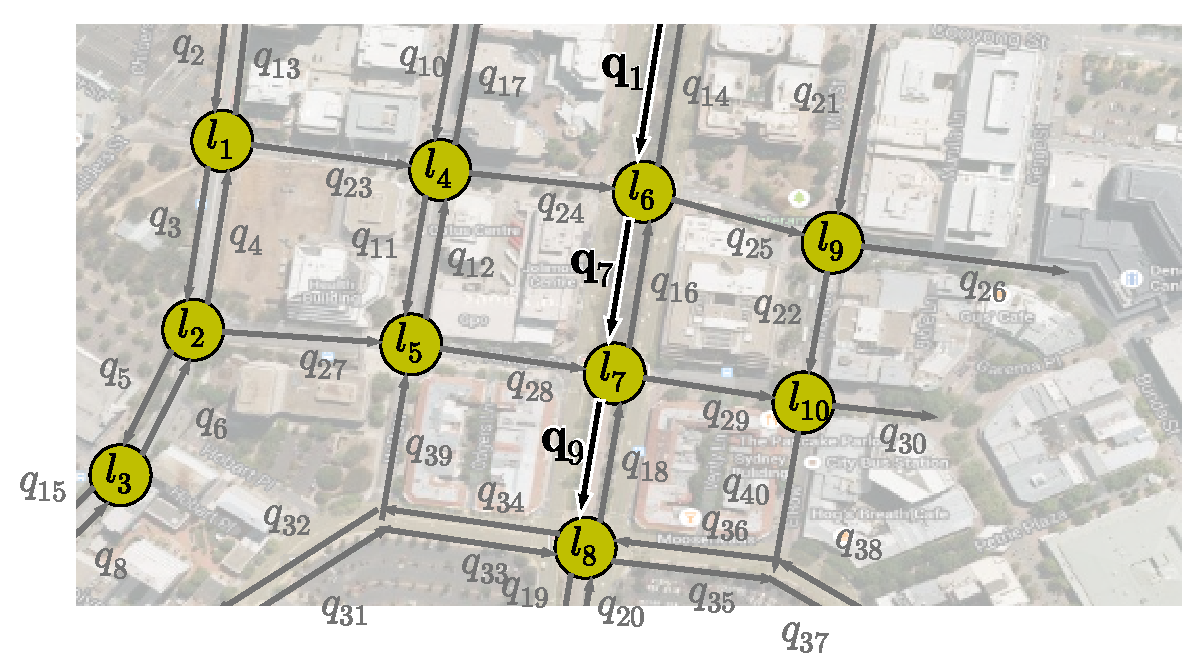
\includegraphics[width=0.5\textwidth,trim={1.3cm 1.1cm 3cm 0.5cm},clip]{map_overlay.pdf}
}
\subfigure[]{
\label{subfig:example}
%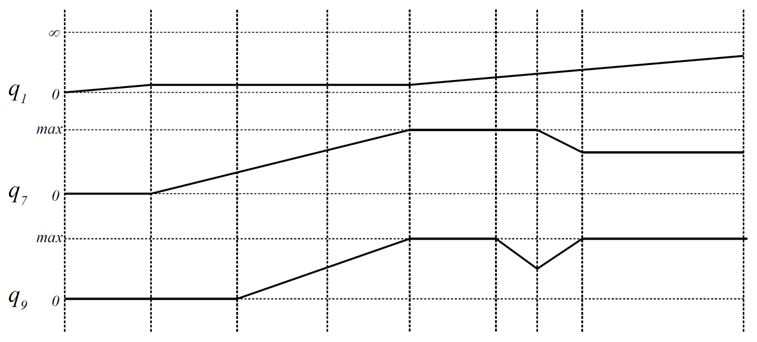
\includegraphics[width=0.45\textwidth,trim={0cm 0cm 0cm 0cm},clip]{map_example.png}
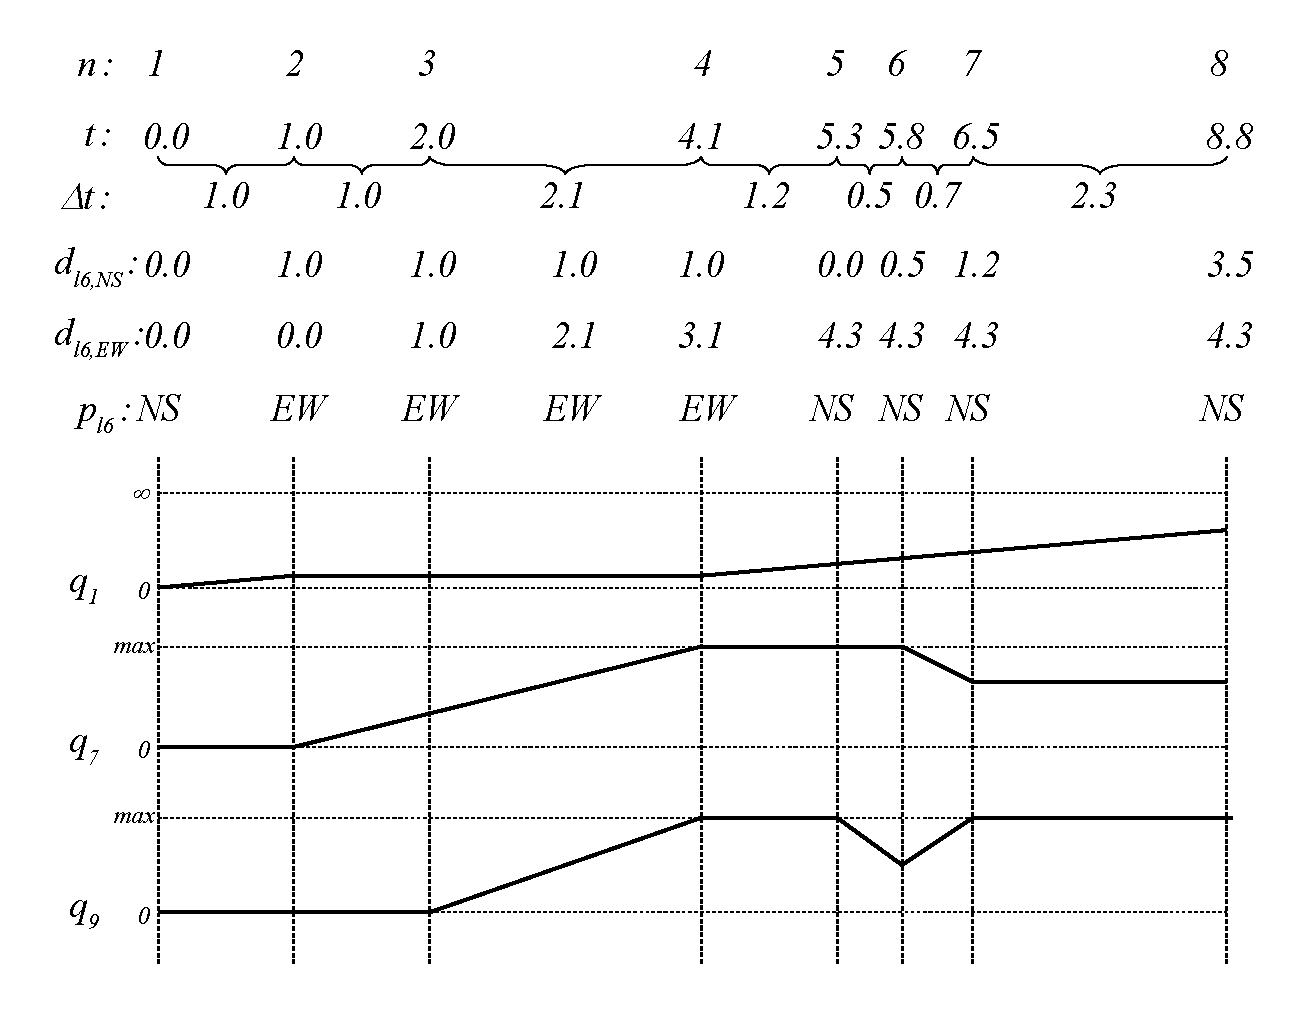
\includegraphics[width=0.44\textwidth,trim={0cm 0cm 0cm 0cm},clip]{plots/pw_queues.pdf}
}
% NOTE: Reviewers like to skim a paper by reading captions so I intentionally
\caption{(a) Example of a real traffic network modeled using the
  QTM. (b) A preview of different QTM model parameters as a function
  of \emph{non-homogeneous} discretized time intervals indexed by $n$.
  For each $n$, we show the following parameters: the elapsed time
  $t$, the non-homogeneous time step length $\Delta t$, the cumulative
  duration $d$ of two different light phases for $l_6$, the phase $p$
  of light $l_6$, and the traffic volume of different queues $q$
  linearly interpolated between time points.  There is technically a
  binary $p$ for each phase, but we abuse notation and simply
  show the current active phase: $\mathit{NS}$ for \emph{north-south green} and 
  $\mathit{EW}$ for \emph{east-west green} assuming the top of the map is north.
  Here we see that traffic progresses from $q_1$ to $q_7$ to $q_9$
  according to light phases and traffic propagation delay with non-homogeneous time steps
  only at required changepoints.
  %Time interval boundaries are only necessary at
  %nonlinear changepoints in queue volume.
  We refer to the QTM model section for
  precise notation and technical definitions.}
\label{fig:qtm}
%
\end{figure*}

For this reason, as a major contribution of this work to enable our
non-homogeneous time MILP-based model of joint intersection control, we
contribute the queue transmission model (QTM) that blends elements of
cell-based and link-based modeling approaches as illustrated
and summarized in Figure~\ref{fig:qtm}.  The QTM offers the following key benefits:
\begin{itemize}
%
\item  Unlike previous CTM-based joint intersection signal 
  optimization~\trbcitenum{lo1998novel,lin2004enhanced,han2012link}, the QTM is
  intended for \emph{non-homogeneous} time steps that can
  be used for control over large horizons.
%
\item Any length of roadway with no merges or diverges can be modeled
  as a single queue leading to compact QTM models of large traffic
  networks thus maintaining relatively compact MILPs
  (i.e., large numbers of cells and their associated MILP variables are
  not required \emph{between} intersections).
%
\item The QTM accurately models fixed travel time delays critical to green wave
  coordination as
  in~\trbcitenum{gartner1974optimization,gartner2002arterial,he2011pamscod}
  through the use of a non-first order Markovian update model and further combines this
  with fully joint intersection signal optimization in the spirit 
  of~\trbcitenum{lo1998novel,lin2004enhanced,han2012link}.
\end{itemize}

In the remainder of this paper, we first formalize our
novel QTM model of traffic flow with non-homogeneous time steps and
show how to encode it as a linear program for computing traffic flows.
%
Next we proceed to allow the traffic signals to become discrete phase
variables that are optimized subject to a delay minimizing objective
and standard minimum and maximum time constraints for cycles and
phases; this results in our final MILP formulation of traffic signal
control.
%
We then experiment with this novel QTM-based MILP control in a range
of traffic networks demonstrating that using non-homogeneous time steps, we can
optimally solve large networks with a fraction of the MILP binary
variables required to achieve the same solution quality with a
homogeneous time step.
%
%We then experiment with this novel QTM-based MILP signal control in a range
%of traffic networks demonstrating substantially improved scalability and
%traffic signal control quality when using non-homogeneous time steps
%in comparison to homogeneous time steps.
%
%We then experiment with this novel QTM-based MILP control in
%a range of networks demonstrating the improved scalability possible
%with non-homogeneous time steps in comparison to homogeneous
%time steps.
%
%These experiments also provide near-optimal traffic control policies
%for larger horizons and larger networks than shown in previous
%implementations of MILP-based traffic signal control.
%\fnremark{ We could really use some pictures in the Intro to refer to
%  here and subsequently -- both a traffic network divided into queues,
%  and the concept of the piecewise linear evolution of traffic flow
%  with {\bf non-homogeneous} (dilated) time steps, something like I had
%  provided in my early writeup.  I think these help visually explain
%  much of the context for the paper and its approach and are critical
%  for reviewer understanding on a time budget for reading this They
%  may only read the first 2-3 pages and then skim!}
%\fnremark{A picture is worth
%  a 1000 words but we only pay 250, hence a 4X ROI on pictures!}

%%%%%%%%%%%%%%%%%%%%%%%%%%%%%%%%%%%%%%%%%%%%%%%%%%%%%%%%%%%%%%%%%%%%%%%%%%
%%%%%%%%%%%%%%%%%%%%%%%%%%%%%%%%%%%%%%%%%%%%%%%%%%%%%%%%%%%%%%%%%%%%%%%%%%
%%%%%%%%%%%%%%%%%%%%%%%%%%%%%%%%%%%%%%%%%%%%%%%%%%%%%%%%%%%%%%%%%%%%%%%%%%

\comment{
optimization techniques as
proposed in various works~\cite (Gartner, Lin and Wang, MARLIN --
Toronto, SURTRAC -- Smith).  In this work, we specifically build on
the MILP approach to traffic optimization that extends previous work
by Lin and Wang who optimize traffic signals (discrete choices at each
time step) in a Cell Transmission Model
(CTM)~\trbcite{daganzo1995cell} of traffic flow.  Unfortunately a CTM
based model is limited in scalability by the requirement that each
road way in the network must be partitioned up into segments that take
exactly $\DT[]=1$ to traverse at the free flow speed.  This leads to a
large number of cells (and hence variables in the MILP) and it makes
it difficult to allow for variable length (non-homogeneous) time steps
in the model updates that we demonstrate in this work to be useful for
optimized traffic signal planning over long horizons.

To allow for more parsimonious models of traffic flow and non-homogeneous
time steps for updates, we introduce the queue transmission model (QTM) [succinct description needed], which offers the following
benefits:
\begin{itemize}
\item non-homogeneous time steps which can keep the model compact over long horizons
\item models platoons without fine-grained cell-based road model or explicit variables to model platoons -- underlies a key precept in urban traffic control to let platoons pass through without stopping,
\item still leads to a MILP, albeit one with much fewer variables owing to the reduced number of queues vs. cells and the reduced number of time steps.
\end{itemize}
Some drawbacks -- does not capture nonlinear flow-density relationship of the
fundamental diagram.  \remark{Argue why this is OK for saturated
  urban networks at peak times.  Green waves in SCATS/SCOOT operate on
  principle of a fixed propagation time, so does Gartner's MILP model.
Captures the right level of detail without blowing up size of model.}
}

%%%%%%%%%%%%%%%%%%%%%%%%%%%%%%%%%%%%%%%%%%%%%%%%%%%%%%%%%%%%%%%%%%%%%%%%%%

\comment{
Lin and Wang aim for network-wide control with a MILP but use
a CTM that requires the time-step to be fixed (otherwise changing
time steps would lead to changing cell sizes and require
dynamic traffic realllocation).

Other GA and reinforcement learning methods, but hard to provide
optimality guarantees.

Much work on optimized traffic control focusing on green-wave
signal coordination given predicted demands and are 
non-homogeneous, but these are largely focused on arterial
control.

Need a deep lookahead possible with non-homogeneous time steps,
but a globally optimized model.  Need to move beyond CTM of
Lin and Wang since this requires fixed time steps, but
still need to model coordination and delays.


Many extensions of CTM for various settings.
...
However, none of these allow non-homogeneous modeling.


To this end we introduce the QTM.  Shares aspects of link-based 
and cell-based models while getting delays right (as in existing
MILP control methosd), but allowing for non-homogeneous time
steps, unlike existing CTMs or extensions.  Ultimately we
will show that a non-homogeneous time step leads to smaller MILPs
and hence improved scalability over a fixed homogeneous time
variant.
}

%%%%%%%%%%%%%%%%%%%%%%%%%%%%%%%%%%%%%%%%%%%%%%%%%%%%%%%%%%%%%%%%%%%%%%%%%%

\comment{

daganzo1994cell - original CTM development

daganzo1995cell - original CTM development

alecsandru2011assessment - general CTM survey noting wide use in many areas

xiaojian2010urban - variable CTM, adjustable cell length

jabari2012stochastic - alternative to CTM for modeling random headways

sumalee2011stochastic - stochastic CTM for modeling mean and standard deviation of traffic flow accurately

muralidharan2009freeway - link-node-CTM, better for arteries+freeway

lu2011discrete - lagged CTM, some sort of improvement

kim2002online - situational CTM, defines more cell types to better model boundary conditions of CTM simulation

huang2011traffic - CTM-Urban, claims CTM was for freeways, and defines extensions to better model urban traffic

gomes2006optimal - assymetric CTM (merge imbalance), freeway ramp metering

MISSING: Knoop et al, Network Transmission Model, more macroscopic variation on CTM, reduces under certain conditions


gartner1974optimization, gartner2002arterial, 

el2013multiagent

Control
===

canepa2012exact - not control, but traffic density estimation

gartner1974optimization - green wave coordination MILP?

gartner2002arterial - green wave coordination MILP?  (OPAC?)

han2012link - link-based MILP (road not divided into cells, criticizes CTM as having too many cells, still approximates shockwaves somehow)

el2013multiagent - MARLIN, pairwise Qlearning

lo1998novel - CTM, MILP introduction

lo1999dynamic - CTM, genetic algorithm solution to MILP

lin2004enhanced - CTM-based MILP

he2011pamscod - optimized solutions to MILP signal coordination (travel-time oriented)

he2014multi - multimodal extensions to MILP signal coordination

he2010heuristic - heuristic solutions to MILP signal coordination

smith2013surtrac - SURTRAC, scheduling for green waves

MISSING other optimized control: Also, PRODYN, RHODES... should ideally include these.
}

%%%%%%%%%%%%%%%%%%%%%%%%%%%%%%%%%%%%%%%%%%%%%%%%%%%%%%%%%%%%%%%%%%%%%%%%%%

\comment{

UNUSED TEXT from shelved grant application draft

Congestion is increasing.

Traffic accounts for X hours of people's time and an improvement
of Y\% would lead to Z amount of dollars saved.

Unfortunately, the majority of urban traffic signal coordination is handled by 
1970's and 1980's era systems that neither make effective use of all
data they collect nor rely on modern optimization techniques to attempt
to find an optimal control policy w.r.t.\ some criteria.

(1) while they collect real-time data, they do not make
use of it in a learning manner to build models of traffic flow, which
can later be optimized, and (2) their techniques for
multi-intersection traffic signal coordination are heuristic and
manually tuned.  In this proposal, we leverage the intersection of two
key technologies that will enable a new generation of traffic
controllers: (a) we now have the algorithms and architectures to
crunch large real-time traffic data for online learning of traffic
models and (b) we now have optimization tools like CPLEX and Gurobi
for mixed integer linear programs (MILPs) that can efficiently solve
large-scale optimization problems that would have been intractable
only a decade ago.  Using these technologies, we aim to use the
real-time (Big) data collected from modern traffic control systems to
build a joint hybrid (switching nonlinear) automata model of traffic
signal control and traffic flow and then to used mixed integer linear
programming techniques to iteratively solve for a provably optimal
control strategy for this automaton.

% Continuous time switching automata contributions... bilinear but
% solve with a splitting approach.

%Questions can be (a) improved traffic light control based on
%real-time predictive models of traffic flow, (b) detection of
%anomalies that should be investigated -- lower than normal flow
%%indicating a potential accident / blocked lane, (c) traffic network
%design for improved flow, (d) incentivizing traffic users by selecting
%transit and parking fares to obtain behavior that improves traffic
%flow.

\blankline

{\bf Intellectual Merit:} %\remark{(verbose for now, compress later)}

\begin{itemize}
\item {\it Modeling traffic control as a (nonlinear switching) hybrid automata}
\item {\it Data-driven hybrid automata learning} 
\item {\it Iterative solving of nonlinear switching hybrid automata with mixed integer linear programming}
\end{itemize}

\blankline

{\bf Broader Impact:}

\begin{itemize}
\item {\it Community:} Publications, but also domains in future IPPCs
  to drive future research and comparison of techniques.
\item {\it Engagement/Impact:} Does Australian engagement count,
  e.g. VicRoads?).
\item {\it Education:} MS and PhD training, competitions, courses,
  workshops and tutorials on traffic and data-driven hybrid automata
  model learning.
\end{itemize}

\blankline

{\bf Key Words:} traffic signal control, hybrid automata, smart cities,
Big Data, machine learning

%%%%%%%%%%%%%%%%%%%%%%%%%%%%%%%%%%%%%%%%%%%%%%%%%%%%%%%%%%%%%%%%%%%%%%%
%% Content from a different proposal on smart cities (power, HVAC, etc)
%%%%%%%%%%%%%%%%%%%%%%%%%%%%%%%%%%%%%%%%%%%%%%%%%%%%%%%%%%%%%%%%%%%%%%%

%We are at the cusp of a new era creating smarter, cleaner, more
%efficient cities that leverage real-time data and online optimization
%to intelligently control everything from traffic signals to heating
%and air conditioning in office buildings to the scheduling of
%industrial and consumer demand to coincide with transient peaks in
%production from green energy sources (solar, wind, etc.).

%The key to achieving these tasks lies in the ability to transform
%complex models containing high degrees of concurrency, hybrid (mixed
%discrete and continuous) state, exogenous events

%learned from large quantities of data into actionable decisions in
%real-time --- a task which requires online optimization at a scale
%and speed unprecented in existing online planning work.

%the bottleneck in using it in real-time stems more from the lack of
%scalable optimization.

%Need to be online.

%Problems are large (concurrent, hybrid) structured, require
%exploitation of that structure beyond naive sampling approaches.

%Existing city infrastructure (coordinating traffic lights, optimal
%heating and air conditioning in buildings, ) often operate in a
%manually controlled or otherwise heuristic settings that do not make
%complete use of real-time data that can be made ava

%Data is now available, optimization techniques can now scale to
%thousand and even millions of variables (with decompositions).

}
